% Created by tikzDevice version 0.11 on 2018-12-11 10:42:14
% !TEX encoding = UTF-8 Unicode
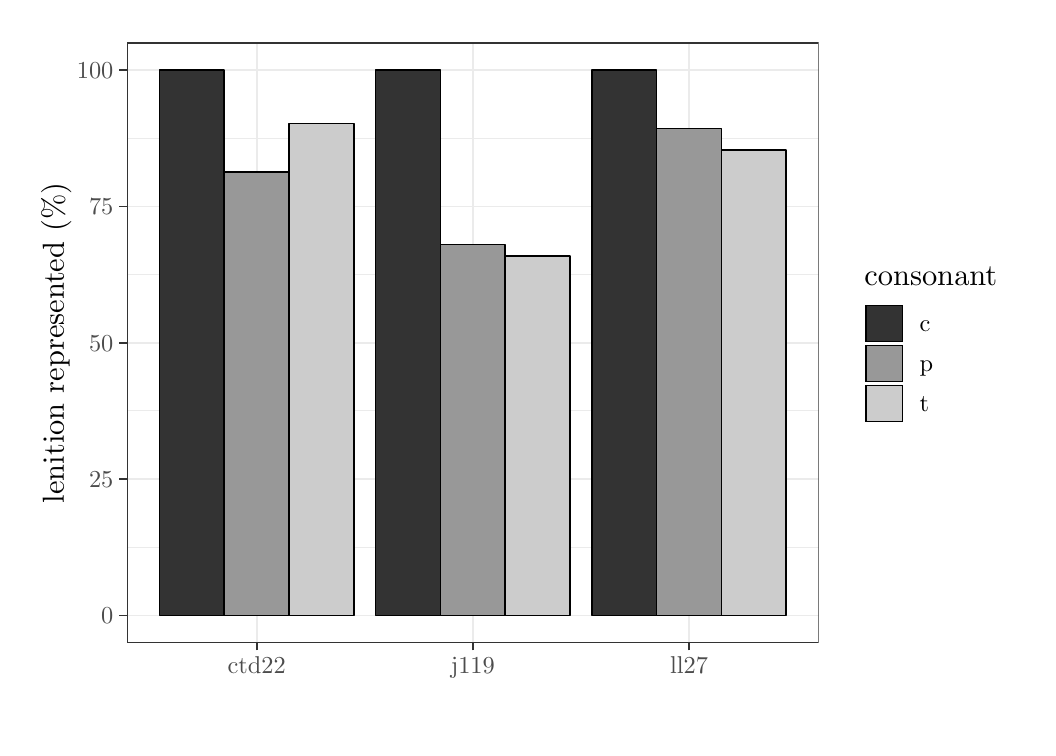
\begin{tikzpicture}[x=1pt,y=1pt]
\definecolor{fillColor}{RGB}{255,255,255}
\path[use as bounding box,fill=fillColor,fill opacity=0.00] (0,0) rectangle (361.35,252.94);
\begin{scope}
\path[clip] (  0.00,  0.00) rectangle (361.35,252.94);
\definecolor{drawColor}{RGB}{255,255,255}
\definecolor{fillColor}{RGB}{255,255,255}

\path[draw=drawColor,line width= 0.6pt,line join=round,line cap=round,fill=fillColor] (  0.00,  0.00) rectangle (361.35,252.94);
\end{scope}
\begin{scope}
\path[clip] ( 35.92, 30.72) rectangle (285.83,247.45);
\definecolor{fillColor}{RGB}{255,255,255}

\path[fill=fillColor] ( 35.92, 30.72) rectangle (285.83,247.45);
\definecolor{drawColor}{gray}{0.92}

\path[draw=drawColor,line width= 0.3pt,line join=round] ( 35.92, 65.20) --
	(285.83, 65.20);

\path[draw=drawColor,line width= 0.3pt,line join=round] ( 35.92,114.46) --
	(285.83,114.46);

\path[draw=drawColor,line width= 0.3pt,line join=round] ( 35.92,163.71) --
	(285.83,163.71);

\path[draw=drawColor,line width= 0.3pt,line join=round] ( 35.92,212.97) --
	(285.83,212.97);

\path[draw=drawColor,line width= 0.6pt,line join=round] ( 35.92, 40.58) --
	(285.83, 40.58);

\path[draw=drawColor,line width= 0.6pt,line join=round] ( 35.92, 89.83) --
	(285.83, 89.83);

\path[draw=drawColor,line width= 0.6pt,line join=round] ( 35.92,139.08) --
	(285.83,139.08);

\path[draw=drawColor,line width= 0.6pt,line join=round] ( 35.92,188.34) --
	(285.83,188.34);

\path[draw=drawColor,line width= 0.6pt,line join=round] ( 35.92,237.59) --
	(285.83,237.59);

\path[draw=drawColor,line width= 0.6pt,line join=round] ( 82.78, 30.72) --
	( 82.78,247.45);

\path[draw=drawColor,line width= 0.6pt,line join=round] (160.87, 30.72) --
	(160.87,247.45);

\path[draw=drawColor,line width= 0.6pt,line join=round] (238.97, 30.72) --
	(238.97,247.45);
\definecolor{drawColor}{RGB}{0,0,0}
\definecolor{fillColor}{gray}{0.80}

\path[draw=drawColor,line width= 0.6pt,line join=round,fill=fillColor] ( 94.49, 40.58) rectangle (117.92,218.29);
\definecolor{fillColor}{RGB}{152,152,152}

\path[draw=drawColor,line width= 0.6pt,line join=round,fill=fillColor] ( 71.06, 40.58) rectangle ( 94.49,200.75);
\definecolor{fillColor}{gray}{0.20}

\path[draw=drawColor,line width= 0.6pt,line join=round,fill=fillColor] ( 47.63, 40.58) rectangle ( 71.06,237.59);
\definecolor{fillColor}{gray}{0.80}

\path[draw=drawColor,line width= 0.6pt,line join=round,fill=fillColor] (172.59, 40.58) rectangle (196.02,170.41);
\definecolor{fillColor}{RGB}{152,152,152}

\path[draw=drawColor,line width= 0.6pt,line join=round,fill=fillColor] (149.16, 40.58) rectangle (172.59,174.55);
\definecolor{fillColor}{gray}{0.20}

\path[draw=drawColor,line width= 0.6pt,line join=round,fill=fillColor] (125.73, 40.58) rectangle (149.16,237.59);
\definecolor{fillColor}{gray}{0.80}

\path[draw=drawColor,line width= 0.6pt,line join=round,fill=fillColor] (250.68, 40.58) rectangle (274.11,208.83);
\definecolor{fillColor}{RGB}{152,152,152}

\path[draw=drawColor,line width= 0.6pt,line join=round,fill=fillColor] (227.26, 40.58) rectangle (250.68,216.51);
\definecolor{fillColor}{gray}{0.20}

\path[draw=drawColor,line width= 0.6pt,line join=round,fill=fillColor] (203.83, 40.58) rectangle (227.26,237.59);
\definecolor{drawColor}{gray}{0.20}

\path[draw=drawColor,line width= 0.6pt,line join=round,line cap=round] ( 35.92, 30.72) rectangle (285.83,247.45);
\end{scope}
\begin{scope}
\path[clip] (  0.00,  0.00) rectangle (361.35,252.94);
\definecolor{drawColor}{gray}{0.30}

\node[text=drawColor,anchor=base east,inner sep=0pt, outer sep=0pt, scale=  0.88] at ( 30.97, 37.55) {0};

\node[text=drawColor,anchor=base east,inner sep=0pt, outer sep=0pt, scale=  0.88] at ( 30.97, 86.80) {25};

\node[text=drawColor,anchor=base east,inner sep=0pt, outer sep=0pt, scale=  0.88] at ( 30.97,136.05) {50};

\node[text=drawColor,anchor=base east,inner sep=0pt, outer sep=0pt, scale=  0.88] at ( 30.97,185.31) {75};

\node[text=drawColor,anchor=base east,inner sep=0pt, outer sep=0pt, scale=  0.88] at ( 30.97,234.56) {100};
\end{scope}
\begin{scope}
\path[clip] (  0.00,  0.00) rectangle (361.35,252.94);
\definecolor{drawColor}{gray}{0.20}

\path[draw=drawColor,line width= 0.6pt,line join=round] ( 33.17, 40.58) --
	( 35.92, 40.58);

\path[draw=drawColor,line width= 0.6pt,line join=round] ( 33.17, 89.83) --
	( 35.92, 89.83);

\path[draw=drawColor,line width= 0.6pt,line join=round] ( 33.17,139.08) --
	( 35.92,139.08);

\path[draw=drawColor,line width= 0.6pt,line join=round] ( 33.17,188.34) --
	( 35.92,188.34);

\path[draw=drawColor,line width= 0.6pt,line join=round] ( 33.17,237.59) --
	( 35.92,237.59);
\end{scope}
\begin{scope}
\path[clip] (  0.00,  0.00) rectangle (361.35,252.94);
\definecolor{drawColor}{gray}{0.20}

\path[draw=drawColor,line width= 0.6pt,line join=round] ( 82.78, 27.97) --
	( 82.78, 30.72);

\path[draw=drawColor,line width= 0.6pt,line join=round] (160.87, 27.97) --
	(160.87, 30.72);

\path[draw=drawColor,line width= 0.6pt,line join=round] (238.97, 27.97) --
	(238.97, 30.72);
\end{scope}
\begin{scope}
\path[clip] (  0.00,  0.00) rectangle (361.35,252.94);
\definecolor{drawColor}{gray}{0.30}

\node[text=drawColor,anchor=base,inner sep=0pt, outer sep=0pt, scale=  0.88] at ( 82.78, 19.71) {\gls{ctd22}};

\node[text=drawColor,anchor=base,inner sep=0pt, outer sep=0pt, scale=  0.88] at (160.87, 19.71) {\gls{j119}};

\node[text=drawColor,anchor=base,inner sep=0pt, outer sep=0pt, scale=  0.88] at (238.97, 19.71) {\gls{ll27}};
\end{scope}
\begin{scope}
\path[clip] (  0.00,  0.00) rectangle (361.35,252.94);
\definecolor{drawColor}{RGB}{0,0,0}

\node[text=drawColor,rotate= 90.00,anchor=base,inner sep=0pt, outer sep=0pt, scale=  1.10] at ( 13.08,139.08) {lenition represented (\%)};
\end{scope}
\begin{scope}
\path[clip] (  0.00,  0.00) rectangle (361.35,252.94);
\definecolor{fillColor}{RGB}{255,255,255}

\path[fill=fillColor] (296.83,104.39) rectangle (355.85,173.78);
\end{scope}
\begin{scope}
\path[clip] (  0.00,  0.00) rectangle (361.35,252.94);
\definecolor{drawColor}{RGB}{0,0,0}

\node[text=drawColor,anchor=base west,inner sep=0pt, outer sep=0pt, scale=  1.10] at (302.33,159.73) {consonant};
\end{scope}
\begin{scope}
\path[clip] (  0.00,  0.00) rectangle (361.35,252.94);
\definecolor{fillColor}{RGB}{255,255,255}

\path[fill=fillColor] (302.33,138.80) rectangle (316.78,153.26);
\end{scope}
\begin{scope}
\path[clip] (  0.00,  0.00) rectangle (361.35,252.94);
\definecolor{drawColor}{RGB}{0,0,0}
\definecolor{fillColor}{gray}{0.20}

\path[draw=drawColor,line width= 0.6pt,line cap=round,fill=fillColor] (303.04,139.51) rectangle (316.07,152.54);
\end{scope}
\begin{scope}
\path[clip] (  0.00,  0.00) rectangle (361.35,252.94);
\definecolor{fillColor}{RGB}{255,255,255}

\path[fill=fillColor] (302.33,124.35) rectangle (316.78,138.80);
\end{scope}
\begin{scope}
\path[clip] (  0.00,  0.00) rectangle (361.35,252.94);
\definecolor{drawColor}{RGB}{0,0,0}
\definecolor{fillColor}{RGB}{152,152,152}

\path[draw=drawColor,line width= 0.6pt,line cap=round,fill=fillColor] (303.04,125.06) rectangle (316.07,138.09);
\end{scope}
\begin{scope}
\path[clip] (  0.00,  0.00) rectangle (361.35,252.94);
\definecolor{fillColor}{RGB}{255,255,255}

\path[fill=fillColor] (302.33,109.89) rectangle (316.78,124.35);
\end{scope}
\begin{scope}
\path[clip] (  0.00,  0.00) rectangle (361.35,252.94);
\definecolor{drawColor}{RGB}{0,0,0}
\definecolor{fillColor}{gray}{0.80}

\path[draw=drawColor,line width= 0.6pt,line cap=round,fill=fillColor] (303.04,110.61) rectangle (316.07,123.64);
\end{scope}
\begin{scope}
\path[clip] (  0.00,  0.00) rectangle (361.35,252.94);
\definecolor{drawColor}{RGB}{0,0,0}

\node[text=drawColor,anchor=base west,inner sep=0pt, outer sep=0pt, scale=  0.88] at (322.28,143.00) {\mw{c}};
\end{scope}
\begin{scope}
\path[clip] (  0.00,  0.00) rectangle (361.35,252.94);
\definecolor{drawColor}{RGB}{0,0,0}

\node[text=drawColor,anchor=base west,inner sep=0pt, outer sep=0pt, scale=  0.88] at (322.28,128.54) {\mw{p}};
\end{scope}
\begin{scope}
\path[clip] (  0.00,  0.00) rectangle (361.35,252.94);
\definecolor{drawColor}{RGB}{0,0,0}

\node[text=drawColor,anchor=base west,inner sep=0pt, outer sep=0pt, scale=  0.88] at (322.28,114.09) {\mw{t}};
\end{scope}
\end{tikzpicture}
